\section{Methods}

Describe the method of solveing. Use MATH6020 project description as a baseline (since its mainly the same method).
Should give enough detail so that this method can be replicated (verbatim psuedo code?).
essentially describing the discritization of M so that it can be solved using finite difference method and how C is solved by trapezidral rule.


%%%%%%%%%%%%%%%%%%%%%%%%%%%%%%%%%%%%%%%%%%%%
\subsection{Substrate Concentration}
  The substrate concentration is represented by the following equation:
  \begin{equation} \label{eq:c=g}
    C_t = g(C,M).
  \end{equation}
  For our case we will use
  \begin{equation} \label{func:g}
    g(C,M) = -\frac{\nu C}{k + C} M.
  \end{equation}
  
  To solve for C we first apply the Fundemental Theorem of Calculus and the Trapizoidal Rule to (\ref{eq:c=g}).
  \begin{equation}
  \begin{aligned}
    \int^{t_{n+1}}_{t_n} C_t dt &= \int^{t_{n+1}}_{t_n} g(C,M) dt \\
    C_{t_{n+1}} - C_{t_n} &= \frac{(t_{n+1} - t_n)}{2} \left( g(C_{t_{n+1}},M_{t_{n+1}}) + g(C_{t_n}, M_{t_n})  \right).
  \end{aligned}
  \end{equation}
  For convience we will henceforth let $C_n = C_{t_n}$, $M_n = M_{t_n}$, and $h = t_{n+1} - t_n$.
  Now we substituite (\ref{func:g}) and try to solve explicitly for $C_{n+1}$
  \begin{equation} \begin{aligned}
    C_{n+1} - C_n &= \frac{h}{2}  \left( -\frac{\nu C_{n+1}}{k + C_{n+1}} M_{n+1}  -\frac{\nu C_n}{k + C_n} M_n \right) \\
    C_{n+1} (k + C_{n+1}) - C_n (k + C_{n+1}) &= -\frac{h}{2} \nu M_{n+1} C_{n+1} - \frac{h}{2} \frac{\nu C_n M_n}{k + C_n} (k + C_{n+1})
  \end{aligned} \end{equation}
  This gives us the following quadratic equation
  \begin{equation}  
    C_{n+1}^2 + \left( k - C_n + \frac{h}{2} \nu M_{n+1} + \frac{h}{2}\frac{\nu C_n M_n}{k + C_n} \right) C_{n+1} + \left( -k C_n + \frac{h}{2} \frac{\nu k C_n M_n}{k + C_n} \right) = 0
  \end{equation}
  from which we can identify
  \begin{equation} \begin{aligned} \label{para:abc}
    a &= 1\\
    b &= k - C_n + \frac{h}{2} \nu M_{n+1} + \frac{h}{2}\frac{\nu C_n M_n}{k + C_n}\\
    c &= -k C_n + \frac{h}{2}\frac{\nu k C_n M_n}{k + C_n}
  \end{aligned}  \end{equation}
  
  We can now solve for $C_{n+1}$ using the quadratic formula
  \begin{equation} \label{eq:Cquad}
    C_{n+1} = \frac{-b \pm \sqrt{b^2 - 4ac}}{2a}
  \end{equation}
  
  To figure out which value of $C_{n+1}$ we use, we test the physical situation in which there are no bacteria consuming the substrate, that is $M= 0$. We expect that the substrate level will remain constant from one timestep to the next which this condition. So when $M = 0$ we have that,
  \begin{equation}
    a = 1, \quad b = k - C_n, \quad c = -k C_n,
  \end{equation} 
  which we can use with (\ref{eq:Cquad}) to get
  \begin{equation} \begin{aligned}
    C_{n+1} &= \frac{- (k - C_n) \pm \sqrt{(k - C_n)^2 - 4 (-k C_n)}}{2} \\
      &= \frac{1}{2} \left( C_n - k \pm \sqrt{k^2 + 2 C_n + C_n^2}\right) \\
      &= \frac{1}{2} \left( C_n - k \pm (k+C_n) \right). \\
  \end{aligned} \end{equation}
  Now, if we use the $'+'$ then $C_{n+1} = C_n$ and if we use the $'-'$ then $C_{n+1} = -k$. Since we cannot have a negative substrate concentration, and we also expected the substrate level to remain constant with these conditions, we can conclude that
  \begin{equation}
    C_{n+1} = \frac{-b + \sqrt{b^2 - 4ac}}{2a}
  \end{equation} 
  where $a,b$, and $c$ are defined in (\ref{para:abc})


%%%%%%%%%%%%%%%%%%%%%%%%%%%%%%%%%%%%%%%%%%%%
\subsection{Biomass Density}
  We need to discritize the following equation, where $M(x,y,t) \equiv M$,
  \begin{equation}
    M_t = \nabla (D(M) \nabla M) + f(C,M) M \\
  \end{equation}
  with respect to both time and space.
  
  First we expand $\nabla(D(M)\nabla M)$,
  \begin{equation}
    M_t = \frac{\partial}{\partial x} \left( D(M) \frac{\partial}{\partial x} M \right) + \frac{\partial}{\partial y} \left( D(M) \frac{\partial}{\partial y} M \right) + f(C,M) M.
  \end{equation}
  
  Now we can discritize for space, (  Note: $D_{i,j} = D(M(x_i,y_j))$) 
  \begin{align}
    M_t &= \frac{1}{\Delta x ^2} \left[ D_{i+\frac{1}{2},j} \left( M_{i+1,j} - M_{i,j}  \right)  - D_{i-\frac{1}{2},j} \left( M_{i,j} - M_{i-1,j}  \right) \right] \\
    &\qquad + \frac{1}{\Delta y ^2} \left[ D_{i,j+\frac{1}{2}} \left( M_{i,j+1} - M_{i,j}  \right)  - D_{i,j-\frac{1}{2}} \left( M_{i,j} - M_{i,j-1}  \right) \right] + f(C,M) M, \notag
  \end{align}

  and also for time,
  \begin{align}
    \frac{M^{n+1} - M^n}{\Delta t} &= \frac{1}{\Delta x ^2} \left[ D_{i+\frac{1}{2},j} \left( M^{n+1}_{i+1,j} - M^{n+1}_{i,j}  \right)  - D_{i-\frac{1}{2},j} \left( M^{n+1}_{i,j} - M^{n+1}_{i-1,j}  \right) \right] \\
    &\qquad + \frac{1}{\Delta y ^2} \left[ D_{i,j+\frac{1}{2}} \left( M^{n+1}_{i,j+1} - M^{n+1}_{i,j}  \right)  - D_{i,j-\frac{1}{2}} \left( M^{n+1}_{i,j} - M^{n+1}_{i,j-1}  \right) \right] \notag \\
    & \qquad + f(C^n,M^n) M^{n+1}.
  \end{align}

  We want to solve this using a linear solver so we rearrange the equation in a form that separates the $M^(n+1)$ terms by their $i,j$-components
  \begin{align}
    \frac{-M^n}{\Delta t} &= \frac{D_{i,j-\frac{1}{2}}}{\Delta y ^2} \cdot M^{n+1}_{i,j-1} + \frac{D_{i-\frac{1}{2},j}}{\Delta x ^2} \cdot M^{n+1}_{i-1,j} \notag \\
    & \qquad +  \left[ -\frac{D_{i,j-\frac{1}{2}}}{\Delta y ^2} - \frac{D_{i-\frac{1}{2},j}}{\Delta x ^2} - \frac{D_{i+\frac{1}{2},j}}{\Delta x ^2} - \frac{D_{i,j+\frac{1}{2}}}{\Delta y ^2} + f(C^n, M^n) - \frac{1}{\Delta t} \right] \cdot M^{n+1}_{i,j} \notag \\
    & \qquad + \frac{D_{i+\frac{1}{2},j}}{\Delta x ^2} \cdot M^{n+1}_{i+1,j} + \frac{D_{i,j+\frac{1}{2}}}{\Delta y ^2} \cdot M^{n+1}_{i,j+1} \notag  \\
        & \qquad + f(C^n,M^n) M^{n+1} \notag \\
  \end{align}
  
  Lastly, multiply both sides by $-1$ for postive definitness
  \begin{align}
    \frac{M^n}{\Delta t} &= \frac{-D_{i,j-\frac{1}{2}}}{\Delta y ^2} \cdot M^{n+1}_{i,j-1} + \frac{-D_{i-\frac{1}{2},j}}{\Delta x ^2} \cdot M^{n+1}_{i-1,j} \notag \\
    & \qquad +  \left[ \frac{D_{i,j-\frac{1}{2}}}{\Delta y ^2} + \frac{D_{i-\frac{1}{2},j}}{\Delta x ^2} + \frac{D_{i+\frac{1}{2},j}}{\Delta x ^2} + \frac{D_{i,j+\frac{1}{2}}}{\Delta y ^2} - f(C^n, M^n) + \frac{1}{\Delta t} \right] \cdot M^{n+1}_{i,j} \notag \\
    & \qquad + \frac{-D_{i+\frac{1}{2},j}}{\Delta x ^2} \cdot M^{n+1}_{i+1,j} + \frac{-D_{i,j+\frac{1}{2}}}{\Delta y ^2} \cdot M^{n+1}_{i,j+1} \notag  
  \end{align}
  
  
  %%%%%%%%%%%%%%%%%%%%%%%%%%%%%%%%%%%%%%%%%



%
%
%
%%%%%%%%%%%%%%%%%%%%%%%%%%%%%%%%%%%
\subsection{Finite Difference Method}
b) \textit{Discretize equation (\ref{equ:darcyElliptic}) on a uniform rectangular grid with step-size $\Delta x = \Delta y = h = 1/n$ on a grid size $n \times m$. Note that this implies $H = m/n$. The gridpoints are $(x_i,y_i)$ with $x_i = ih,\ i = 0,1,\ldots, n$ and $y_j = jh,\ j = 0,1,\ldots,m.$ To this end, discretize equation (\ref{equ:darcyElliptic}) to obtain a sparse linear system of the form
\begin{equation}
    A p = b,
\end{equation}
where the matrix A can be stored in sparse diagonal format.}

\vspace{0.3cm}
\noindent \underline{\textbf{Answer:}}

To discretize equation (\ref{equ:darcyElliptic}) we first need to create our grid. For this problem we use an orthogonal uniform grid for simplicity. From this we get that our grid points are $(x_i, y_j)$, with $x_i = \frac{i}{n},\ i = 0,1,\ldots, n$ and  $y_j = \frac{j}{m},\ j = 0,1,\ldots, m$. We can approximate (\ref{equ:darcyElliptic}) at a grid point $(i,j)$ as
\begin{equation} \label{equ:intPoint}
\begin{aligned}
    \frac{1}{\Delta t^2} &\left[ k_{i,j-1/2} p_{i,j-1} + k_{i-1/2,j}  p_{i-1,j} \right. \\
    &- \left( k_{i,j-1/2} +k_{i-1/2,j} + k_{i+1/2,j} + k_{i,j+1/2} \right)  p_{i,j} \\
    &\left.+ k_{i+1/2,j} p_{i+1,j}  + k_{i,j+1/2} p_{i,j+1}  \right] = k_{i,j} p_{i,j},
\end{aligned}
\end{equation}
where $k_{i\pm1/2,j\pm1/2} = k(x_i\pm \frac{h}{2},y_j\pm \frac{h}{2})$.

This means that at each grid point $(i,j)$, we have dependency on $p_{i,j}, p_{i\pm1,j}$, and $p_{i,j\pm1}$. This results in a system of $N = nm$ linear equations for $N$ unknown $p_{i,j}$.

Each interior point can be computed using (\ref{equ:intPoint}). For the Boundary points we take special considerations. At $x = 0$ and $x = 1$ we have Dirichlet Boundary Conditions. These grid points are excluded from the matrix computations since their values are known. At $y=0$ and $y=1$ we have Neumann Boundary Conditions. For these a second order approximation of the derivative is used. 

\begin{figure}[htb]
  \begin{center}
    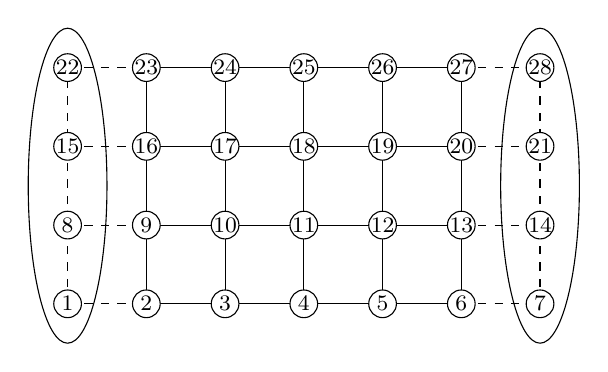
\begin{tikzpicture}[scale = 1.00]
        \draw (1,0) grid  (5,3);
        \draw [dashed] (0,0) grid (1,3);
        \draw [dashed] (5,0) grid (6,3);
        
        \draw (0,1.5) ellipse (.5cm and 2cm);
        \draw (6,1.5) ellipse (.5cm and 2cm);
        
        
        \draw [fill=white] (0,0) circle [radius = 5pt];
        \node     at (0,0) {\footnotesize{1}};
        \draw [fill=white] (1,0) circle [radius = 5pt];
        \node     at (1,0) {\footnotesize{2}};
        \draw [fill=white] (2,0) circle [radius = 5pt];
        \node     at (2,0) {\footnotesize{3}};
        \draw [fill=white] (3,0) circle [radius = 5pt];
        \node     at (3,0) {\footnotesize{4}};
        \draw [fill=white] (4,0) circle [radius = 5pt];
        \node     at (4,0) {\footnotesize{5}};
        \draw [fill=white] (5,0) circle [radius = 5pt];
        \node     at (5,0) {\footnotesize{6}};
        \draw [fill=white] (6,0) circle [radius = 5pt];
        \node     at (6,0) {\footnotesize{7}};

        \draw [fill=white] (0,1) circle [radius = 5pt];
        \node     at (0,1) {\footnotesize{8}};
        \draw [fill=white] (1,1) circle [radius = 5pt];
        \node     at (1,1) {\footnotesize{9}};
        \draw [fill=white] (2,1) circle [radius = 5pt];
        \node     at (2,1) {\footnotesize{10}};
        \draw [fill=white] (3,1) circle [radius = 5pt];
        \node     at (3,1) {\footnotesize{11}};
        \draw [fill=white] (4,1) circle [radius = 5pt];
        \node     at (4,1) {\footnotesize{12}};
        \draw [fill=white] (5,1) circle [radius = 5pt];
        \node     at (5,1) {\footnotesize{13}};
        \draw [fill=white] (6,1) circle [radius = 5pt];
        \node     at (6,1) {\footnotesize{14}};
        
        \draw [fill=white] (0,2) circle [radius = 5pt];
        \node     at (0,2) {\footnotesize{15}};
        \draw [fill=white] (1,2) circle [radius = 5pt];
        \node     at (1,2) {\footnotesize{16}};
        \draw [fill=white] (2,2) circle [radius = 5pt];
        \node     at (2,2) {\footnotesize{17}};
        \draw [fill=white] (3,2) circle [radius = 5pt];
        \node     at (3,2) {\footnotesize{18}};
        \draw [fill=white] (4,2) circle [radius = 5pt];
        \node     at (4,2) {\footnotesize{19}};
        \draw [fill=white] (5,2) circle [radius = 5pt];
        \node     at (5,2) {\footnotesize{20}};
        \draw [fill=white] (6,2) circle [radius = 5pt];
        \node     at (6,2) {\footnotesize{21}};
        
        \draw [fill=white] (0,3) circle [radius = 5pt];
        \node     at (0,3) {\footnotesize{22}};
        \draw [fill=white] (1,3) circle [radius = 5pt];
        \node     at (1,3) {\footnotesize{23}};
        \draw [fill=white] (2,3) circle [radius = 5pt];
        \node     at (2,3) {\footnotesize{24}};
        \draw [fill=white] (3,3) circle [radius = 5pt];
        \node     at (3,3) {\footnotesize{25}};
        \draw [fill=white] (4,3) circle [radius = 5pt];
        \node     at (4,3) {\footnotesize{26}};
        \draw [fill=white] (5,3) circle [radius = 5pt];
        \node     at (5,3) {\footnotesize{27}};
        \draw [fill=white] (6,3) circle [radius = 5pt];
        \node     at (6,3) {\footnotesize{28}};
        
        
    \end{tikzpicture}
    \caption{An example of the grid ordering on an 7 x 4 grid.}
    \label{graph:gridordering}
  \end{center}
\end{figure}


To solve this system, the problem is converted into the form
\begin{equation}
  \mathcal{A} p = b
\end{equation}
where $\mathcal{A}$ is the coefficents for each grid point, $p$ is the solution vector, and $b$ is the boundary conditions. To compute this a bijective mapping to convert the 2D grid into a 1D array is required, the following mapping is used here,
\begin{equation}
  \begin{aligned}
    \pi : \{0,\ldots, n\} \times \{0, \ldots, m \} &\to \{ 1, \ldots, (n+1)(m+1) \} \\
          (i,j) \qquad \qquad &\mapsto  \quad \qquad \pi(i,j)
  \end{aligned}
\end{equation}
An example of this grid ordering can be seen in Figure \ref{graph:gridordering}.

\begin{figure}[h!tb]
  \begin{center}
    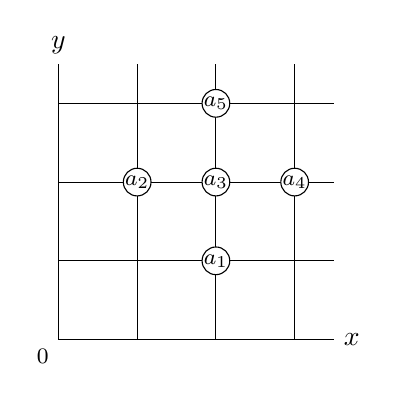
\begin{tikzpicture}[scale = 1.00]
        \draw (-1,-1) grid (1,2.5);
        \draw (1,-1) grid (2.5,2.5);
        
        \node [below left] at (-1,-1) {\footnotesize{0}};
        \node [right] at (2.5,-1) {$x$};
        \node [above] at (-1,2.5) {$y$};
        
        \draw [fill=white] (1,1) circle [radius = 5pt];
        \node at (1,1) {\footnotesize{$a_3$}};
        \draw [fill=white] (0,1) circle [radius = 5pt];
        \node at (0,1) {\footnotesize{$a_2$}};
        \draw [fill=white] (1,0) circle [radius = 5pt];
        \node at (1,0) {\footnotesize{$a_1$}};
        \draw [fill=white] (2,1) circle [radius = 5pt];
        \node at (2,1) {\footnotesize{$a_4$}};
        \draw [fill=white] (1,2) circle [radius = 5pt];
        \node at (1,2) {\footnotesize{$a_5$}};
        
    \end{tikzpicture}
    \caption{A visual of the grid point dependency and their numbering for the diagonally formatted matrix}
    \label{graph:numbering}
  \end{center}
\end{figure}

The matrix is stored in diagonal format and since there are five unknowns for each linear equation the matrix will be banded with five diagonals. The numbering of these diagonals in the matrix can be seen in Figure \ref{graph:numbering} 


